\DiaryEntry{Numerical Linear Algebra, Projections}{2019-10-28}{Linear Algebra}

A \emph{projector} is a square matrix being idempotent; i.e.

\bee
\Pbf^2 = \Pbf
\eee

The projector takes a vector$\xbf$ and projects it onto the subspace being the range of $\Pbf$: $\vbf = \Pbf \xbf$. Projecting again does not change anything; as we have

\bee
\Pbf (\Pbf \xbf) = \Pbf^2 \xbf = \Pbf \xbf = \vbf
\eee

If $\Pbf$ is a projector, then $\Ibf - \Pbf$ is also a projector for we have

\bee
(\Ibf - \Pbf)^2 = \Ibf - 2\Ibf\Pbf + \Pbf^2 = \Ibf - 2\Pbf + \Pbf = \Ibf - \Pbf
\eee

The projector $\Ibf - \Pbf$ projects onto the nullspace of $\Pbf$ and is called the complementary projector. It is called this way, because range and nullspace are complementary, we have

\bee
\text{range}(\Pbf) \cap \text{null}(\Pbf) = \zerobf
\eee

We can write this as

\bee
\Pbf \xbf + (\Ibf - \Pbf) \xbf = \xbf
\eee


We also say that $\Pbf$ projects onto $\text{range}(\Pbf)$ along $\text{null}(\Pbf)$.




\subsection{Orthogonal Projectors}

An orthogonal projector is a projector that projects onto a subspace $S_1$ along a space $S_2$ where $S_1$ and $S_2$ are orthogonal. Expressed algebraically, this amounts to $\Pbf^H = \Pbf$.

If we have an orthonormal basis (expressed as column vectors in $\Qbf$), then a projector onto the subspace spanned by this basis is

\bee
\Pbf = \Qbf \Qbf^H
\eee

The following Figure shows the defintion graphically.

\begin{figure}[hbt!]
\centering
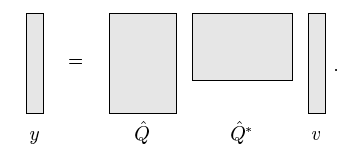
\includegraphics[scale=0.5]{images/num_lin_algebra_04_1.png}
\end{figure}

We can interpret the projection $\Qbf \Qbf^H \xbf$ as follows: First we calculate the inner products of the columns of $\Qbf$ with $\xbf$ (that's $\Qbf^H \xbf$) and then scaling the column vectors of $\Qbf$ by these inner products.

A special case is the projection onto one vector; in this case it is a rank-one orthogonal projector, given by

\bee
\Pbf = \qbf \qbf^H
\eee

\paragraph{Example.} Consider a 2-dimensional subspace in a 3-dimensional space defined by

\bee
\Qbf = \begin{pmatrix} 1 & 0 \\ 0 & 1 \\ 0 & 0 \end{pmatrix}
\eee

Our projector then becomes

\bee
\Pbf = \begin{pmatrix} 1 & 0 & 0 \\ 0 & 1 & 0 \\ 0 & 0 & 0 \end{pmatrix}
\eee

This projector takes the first two coordinates unchanged and sets the third one to zero; i.e.

\bee
\Pbf [v_1 \, v_2 \, v_3]^T = [v_1 \, v_2 \, 0]^T
\eee

A bit more complex and interesting is the following case

\bee
\Qbf = \frac{1}{\sqrt{2}} \begin{pmatrix} 1 & -1 \\ 1 & 1 \\ 0 & 0 \end{pmatrix}
\eee

which yields the following projector

\bee
\Pbf = \begin{pmatrix} 1 & 0 & 0 \\ 0 & 1 & 0 \\ 0 & 0 & 0 \end{pmatrix}
\eee

This is the same projector as before because it is the same subspace we are projecting to (although defined by different basis vectors). 


\subsection{Projection onto an Arbitrary Basis}

We can also project onto a subspace defined by an arbitrary basis which need not be orthogonal. Suppose the subspace is spanned by $N$ vectors $\abf_i$ which are collected column-wise into a matrix $\Abf$. If we project a vector $\vbf$ onto the subspace (yielding $\ybf$), the remainder $\ybf - \vbf$ must be orthogonal to the subspace. We have

\bee
\abf_j^H (\ybf - \vbf)^H = 0, \quad j=1 \ldots N
\eee

We next note that we write $\ybf = \Abf \xbf$ (since $\ybf$ lies in the subspace spanned by $\abf$), and we therefore have

\bee
\abf_j^H(\Abf \xbf - \vbf) = 0, \quad j=1 \ldots N
\eee

Now we combine these $N$ inner products into one expression and obtain

\bee
\Abf^H (\Abf \xbf - \vbf) = 0 \rightarrow \Abf^H \Abf \xbf = \Abf^H \vbf
\eee

From this we can calculate $\xbf$ as

\bee
\xbf = (\Abf^H \Abf)^{-1} \Abf^H \vbf
\eee

and $\ybf$ according to

\bee
\ybf = \Abf \xbf = \Abf (\Abf^H \Abf)^{-1} \Abf^H \vbf
\eee

The projector is therefore

\bee
\Pbf = \Abf (\Abf^H \Abf)^{-1} \Abf^H
\eee


Note that this is equal to the least-squares estimator. This is obtained by noting that the LS estimator minimizes the distance between the observaton and a linear combination of (basis) vectors. The minimum is obtained when the observation is projected onto the subspace defined by the (basis) vectors.

\paragraph{Example.} As an example, we consider the matrix

\bee
\Abf = \begin{pmatrix} 1 & 1 \\ 0 & 1 \\ 0 & 0 \end{pmatrix}
\eee

Note that these vectors are linearly independent, but not orthonormal. The projector is

\bee
\Pbf = \Abf (\Abf^H \Abf)^{-1} \Abf^H = \begin{pmatrix} 1 & 0 & 0 \\ 0 & 1 & 0 \\ 0 & 0 & 0 \end{pmatrix}
\eee

This yields the same projector as before; the whole prcedure ``magically'' produced the same result with non-orthonormal vectors as input.


Projections, QR Factorization, Gram-Schmidt, Gaussian Elimination, Eigenvalues?

%%% Local Variables:
%%% mode: latex
%%% TeX-master: "journal"
%%% End:
